\chapter{Wasserfallmodell mit Rücksprung}
\section{Definition}
\begin{quote}
Das Wasserfallmodell ist ein lineares (nicht iteratives) vorgehensmodell in der Softwareentwicklung, bei dem der
 Sotwareentwicklungsprozess in Phasen organisiert wird. Dabei gehen die Phasenergebnisse wie bei einem Wasserfall immmer
als bindende Vorgaben für die nächsttiefere Phase ein.\ \\ \\
Im Wasserfallmodell hat jede Phase vordefinierte Start- und Endpunkte mit eindeutig definierten Ergebnissen.
In Meilensteinsitzungen am jeweiligen Phasenende werden die Ergenisdokumente verabschiedet. Zu den wichtigsten
Dokumenten zählen dabei das Lastenheft sowie das Pflichenheft. In der betrieblichen Praxis gibt es viele Varianten
des reinen Modells. Es ist aber das traditionell am weitesten verbreitete Vorgehensmodell.\ \\ \\
Der Name \"Wasserfall\" kommt von der häufig gewählten grafischen Darstellung der fünf bis sechs als Kaskade
angeordneten Phasen. Ein erweitertes Wasserfallmodell mit Rücksprungmöglichkeiten (gestrichelt).\ \\ \\
Erweiterungen des einfachen Modells (Wasserfallmodell mit Rücksprung) führen iterative Aspekte ein und erlauben
ein schrittweises \"Aufwärtslaufen\" der Kaskade, sofern in der aktuellen Phase etwas schieflaufen sollte,
um den Fehler auf der nächsthöheren Stufe beheben zu können.
\footnote{Zitat aus:  http://de.wikipedia.org/wiki/Wasserfallmodell}
\end{quote}
\begin{figure}[h]
\centering
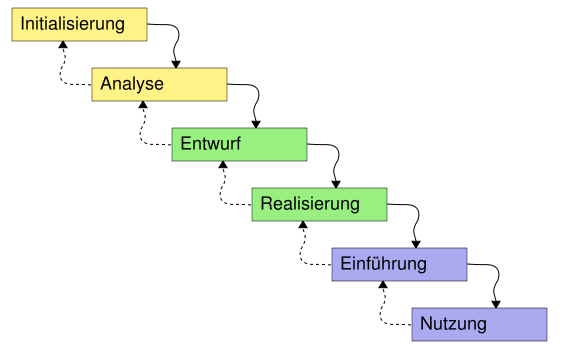
\includegraphics[scale=0.35]{567px-Wasserfallmodell.png}
\end{figure}
\footnote{Wasserfallmodell mit Rücksprung, \\ Bild-Quelle: http://upload.wikimedia.org/wikipedia/commons/thumb/e/e5/Wasserfallmodell.svg/567px-Wasserfallmodell.svg.png}
\section{Warum dieses Modell?}
Wir haben uns für das Wasserfallmodell mit Rücksprung entschieden, weil dieses Modell alle Phasen der 
Entwicklung klar abgrenzt und sich optimal auf einen professionellen Softwareentwicklungsvorgang
abbilden lässt. Dieses Modell ermöglicht eine klare Planung und Kontrolle unseres Softwareprojekts,
da die Anforderungen stets die gleichen bleiben und der Umfang einigermaßen gut abschätzbar ist.
Für die erweiterte Version dieses Modells, nämlich mit Rücksprung, haben wir uns entschieden, um ein 
paar Nachteile dieses Modells auszuhebeln. Beispielsweise sind die klar voneinander abgegrenzten Phasen
in der Realität oft nicht umsetzbar. Des weiteren sind wir somit flexibler gegenüber Änderungen.
\section{Tatsächliche Umsetzung}
Im Laufe der Entwicklung mussten wir feststellen, dass das Wasserfallmodell als Vorgehensweise für unser
Projekt doch nicht so gut geeignet war wie wir erwarteten. Da das Projekt eine viel zu komplexe Infrastruktur
besitzt, die wir vorher unmöglich abschätzen konnten, war es unmöglich zu planen, welcher Arbeitsaufwand nötig ist.
Somit konnten keine brauchbaren Entwürfe der Software gemacht werden, da man sich manche Funktionen des MPD
völlig anders vorgestellt hatte, als sie in Wirklichkeit funktionierten. Daher mussten wir, nachdem
das Lasten- und Pflichtenheft fertiggestellt waren (welche unabhängig von der Infrastruktur sind)), auf agile
Entwicklungsmethoden umschwänken. Aufgrund der hohen Komplexität der MPD Libraries war es uns nicht möglich
sich einen Überblick über interne Abläufe zu verschaffen so mussten wir parallel zu den eigentlichen Planungen
erste Testanwendungen schrieben um sich mit der Materie vertraut zu machen.
Als Beispiel sei hier der Testclient genannt, der letzlich auch die Grundlage für die heutige
Architektur darstellt, bzw. die Grundlage aus der sie entstanden ist.

(TODO: Spiralmodell?)